\chapter{Implementación}
En esta sección se detalla la implementación de este trabajo, que se dividió en dos componentes principales. Primero, se implementó un sistema de inferencia para type-based declassification. Segundo, se elaboró un plugin para editores de texto que integra el resultado de la inferencia.

\section{Lenguaje Dart}
Dart es un lenguaje de programación de propósito general, orientado a objetos y de código abierto desarrollado por Google. Es usado para construir aplicaciones web, móviles y dispositivos IoT (Internet of Things).

La implementación de este trabajo fue realizada en Dart, debido a que proporciona las herramientas necesarias para realizar el análisis requerido, como el AST (Abstract Syntax Tree) resuelto con la información completa de tipos. Además, los investigadores que realizaron el trabajo de \textit{type-based declassification} estudian este lenguaje como parte de un proyecto de investigación mayor en el área de seguridad.

\subsection{Dart Analyzer}
\emph{Dart Analyer} es una herramienta incluida en Dart, que permite realizar análisis estático de código Dart. Entre otros servicios, esta herramienta permite obtener el AST de un código Dart. Dicho AST contiene la información relevante del programa, incluyendo el resultado del análisis de tipos.

Análisis personalizados de programas en Dart pueden ser realizados usando la información del AST. Para facilitar su integración, Dart Analyzer utiliza el patrón Visitor para incorporar un nuevo análisis sobre el AST.

\subsection{Analyzer Plugin}
La herramienta \emph{Analyzer Plugin} sirve para integrar un análisis personalizado sobre el AST generado por Dart Analyzer, con los IDE que tengan soporte para servidores de análisis estático de Dart, como IntelliJ, Eclipse, Atom, entre otros. Con esta librería es posible generar errores, \textit{warnings}, sugerencias de edición, sugerencias de navegación  y resaltado de sintaxis.

\section{Implementación de sistema de inferencia}

\subsection{Representación de facetas públicas}
Para declarar las facetas públicas, se usan las anotaciones de Dart. Por ejemplo,

 \texttt{@S("Top") bool check(@S("StringCompareTo") String password);}

 es una declaración de un método de Dart anotado con facetas públicas.

La definición de las facetas públicas se hace mediante clases abstractas de Dart. Por ejemplo, la faceta \texttt{StringCompareTo} se define mediante la clase abstracta del mismo nombre:

\begin{lstlisting}
  abstract class StringCompareTo {
    int compareTo(String other);
  }
\end{lstlisting}

Antes de la generación de constraints sobre un archivo, se realiza una etapa de \textit{parsing} de facetas públicas, en donde se leen las clases abstractas del archivo. Esto se implementa mediante el \emph{visitor} \texttt{DeclaredFacetVisitor}, que se muestra en el diagrama de la figura \ref{uml}. Las facetas públicas procesadas se almacenan en el diccionario \texttt{declaredStore}, en donde se asocia el nombre de la faceta con su tipo de objeto correspondiente.

\subsection{Tipos de errores}
Durante el proceso de inferencia, se pueden generar varios tipos de errores, los cuales difieren en el mensaje que será desplegado en la interfaz de usuario, y el resaltado que aplicarán en la ubicación correspondiente del código fuente.

\begin{itemize}
  \item \texttt{FlowError:} Se genera por la presencia de una constraint con una relación de subtyping no válida, que no proviene de invocación a método. Es un error, por lo que aplica un resaltado de color rojo en la ubicación correspondiente.
  \item \texttt{WellFormedTypeError:} Se genera por la detección de tipos que no son well-formed. Es un error, por lo que aplica un resaltado de color rojo en la ubicación correspondiente.
  \item \texttt{UndefinedFacetWarning:} Se genera por la declaración de una faceta pública que no ha sido definida. Es un warning, por lo que aplica un resaltado de color amarillo en la ubicación correspondiente.
  \item \texttt{UnableToResolveInfo:} Se genera por la incapacidad de inferir un tipo concreto para una variable de tipo. Es de caracter informativo, por lo que solo aplica un leve resaltado de sintaxis en el código, y muestra un mensaje cuando el cursor se posiciona sobre la ubicación correspondiente.
  \item \texttt{InferredFacetInfo:} Se genera en toda expresión que no posee una faceta pública declarada, con la información de la faceta inferida. Al igual que el tipo de error anterior, es de carácter informativo.
\end{itemize}

\subsection{Fase de generación de constraints}
Una vez que se procesan las facetas públicas, se procede a la generación de constraints. Esto se realiza implementando varios visitors mostrados en el diagrama de la figura \ref{uml}.

La clase encargada de procesar un archivo es \texttt{CompilationUnitVisitor}, en donde se procesa cada clase declarada en el archivo. Mediante el visitor \texttt{ClassMemberVisitor}, se procesa cada método, campo y constructor de cada clase. Finalmente, el visitor implementado para procesar el cuerpo de cada miembro es \texttt{BlockVisitor}, en donde se procesa cada expresión relevante para el algoritmo de generación de constraints de la sección \ref{propuestaGen}.

La clase \texttt{Store} es la encargada de la generación de variables de tipo, y el almacenamiento en diccionarios del tipo de las expresiones. Cada visita a los nodos del AST puede agregar constraints al set de constraints, y agregar o actualizar elementos en el store. Ambos se muestran en el diagrama \ref{uml}.

En esta fase se pueden generar errores de tipo \texttt{WellFormedTypeError} y \texttt{UndefinedFacetWarning}, los cuales son recolectados mediante un \texttt{ErrorCollector}, el cual será utilizado para el despliegue de la información mediante el plugin.

\subsection{Fase de resolución de constraints}
En esta fase, la clase \texttt{ConstraintSolver}, que se muestra en el diagrama \ref{uml}, se encarga de convertir el set de constraints en un mapeo entre variables de tipos y tipos concretos, implementando las operaciones descritas en la sección \ref{propuestaRes}.

Los errores que son generados pueden ser de los tipos \texttt{SubtypingError}, \texttt{UnableToResolveInfo} y \texttt{InferredFacetInfo}, los cuales son recolectados mediante el mismo \texttt{ErrorCollector} de la fase de generación de constraints.

\begin{figure}[ht]
  \centering
  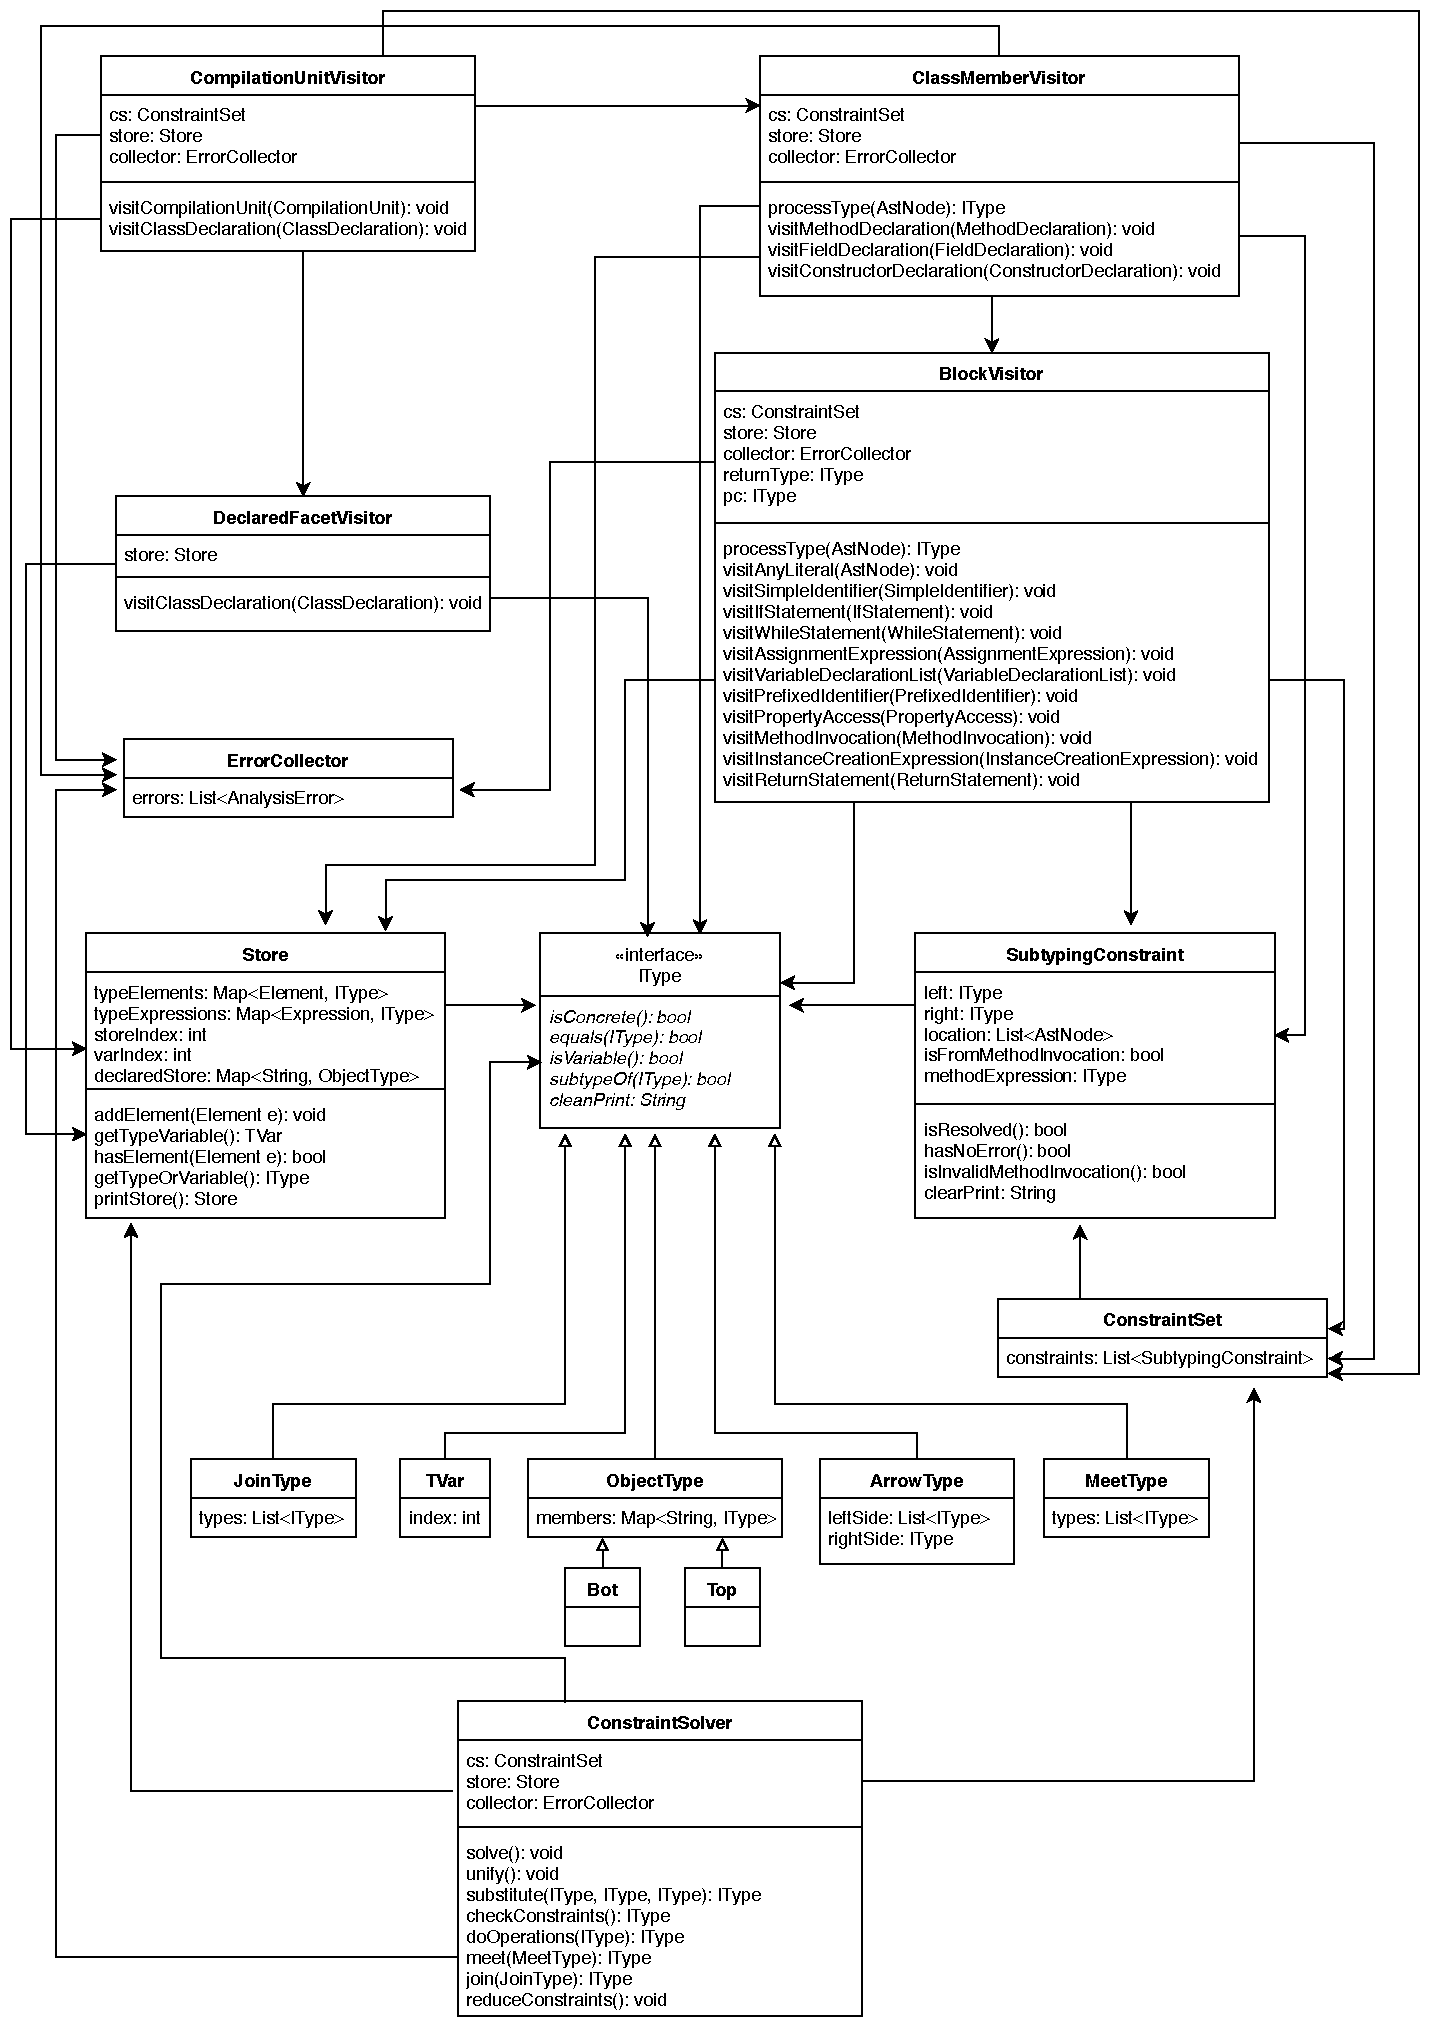
\includegraphics[width=0.93\textwidth]{imagenes/others.pdf}
  \caption{Diagrama de clases de sistema de inferencia}
  \label{uml}
\end{figure}
\clearpage

\section{Implementación de plugin}

\subsection{Descripción general}
Para la implementación del plugin se necesita implementar una API para establecer comunicación con el servidor de análisis de un IDE, respondiendo con el análisis de inferencia ante las peticiones recibidas desde el servidor.

Cuando el servidor de análisis detecta un cambio en un archivo, envía un mensaje al plugin, el cual gatilla la inferencia para todos los archivos del proyecto activo. Además, el plugin se encarga de recolectar los errores generados en las fases del proceso de inferencia, para enviárselos al servidor de análisis, el cual los despliega ante el usuario.

Para la implementación de la API, se siguió el tutorial oficial de la herramienta Analyzer Plugin, presente en el repositorio de GitHub oficial del lenguaje Dart~\cite{plugin}.

\subsection{Configuración del plugin}
Para activar el análisis sobre un proyecto, se debe agregar el paquete del plugin como dependencia al proyecto, y agregar el plugin al archivo de configuración del análisis del proyecto \texttt{analysis\_options.yaml}, ubicado en la raiz del proyecto.

\begin{verbatim}
  analyzer:
    plugins:
      TRNIdart:
        default_core_return: Bot
        default_core_parameter: Bot
\end{verbatim}

Las opciones \texttt{default\_core\_return} y \texttt{default\_core\_parameter} corresponden a las facetas públicas por defecto que tendrán los métodos del \textit{core} de Dart.
